\documentclass[conference]{IEEEtran}
\usepackage{natbib}
\usepackage{url}
\usepackage{hyperref}
\usepackage{framed}
\usepackage{tcolorbox}
\ifCLASSINFOpdf

\else

\fi

\hyphenation{op-tical net-works semi-conduc-tor}


\begin{document}

\title{\textbf{Roamify: Roaming Redefined}\\ \textit{Changing the Way World Travels}}


\author{\IEEEauthorblockN{Vikranth Udandarao}
\IEEEauthorblockA{Computer Science Engineering Dept\\
IIIT Delhi\\
vikranth22570@iiitd.ac.in}
\and
\IEEEauthorblockN{Noel Abraham Tiju}
\IEEEauthorblockA{Computer Science Engineering Dept\\
IIIT Delhi\\
noel22338@iiitd.ac.in}
\and
\IEEEauthorblockN{Muthuraj Vairamuthu}
\IEEEauthorblockA{Computer Science Engineering Dept\\
IIIT Delhi\\
muthuraj22307@iiitd.ac.in}
\and
\IEEEauthorblockN{Harsh Mistry}
\IEEEauthorblockA{Computer Science Engineering Dept\\
IIIT Delhi\\
harsh22200@iiitd.ac.in}
\and
\IEEEauthorblockN{Armaan Singh}
\IEEEauthorblockA{Computer Science Engineering Dept\\
IIIT Delhi\\
armaan22096@iiitd.ac.in}
\and
\IEEEauthorblockN{Dhruv Kumar}
\IEEEauthorblockA{Computer Science Engineering Dept\\
IIIT Delhi\\
dhruv.kumar@iiitd.ac.in}}




% \author{\IEEEauthorblockN{Vikranth Udandarao\IEEEauthorrefmark{1},
% Harsh Mistry\IEEEauthorrefmark{1},
% Muthuraj Vairamuthu\IEEEauthorrefmark{1},
% Noel Tiju\IEEEauthorrefmark{1},
% Armaan Singh\IEEEauthorrefmark{1}}
% \IEEEauthorblockA{\IEEEauthorrefmark{1}Computer Science Engineering Dept\\
% IIIT Delhi\\
% }}




\maketitle

\begin{abstract}

    Travel planning is difficult and time-consuming. AI-driven itinerary plugin Roamify simplifies this by making curated suggestions based on user interests. Roamify uses powerful NLP to parse text from web scraping. LLMs create individualized travel itineraries from processed data. Roamify's methods could convert vacation planning from logistical obstacles to exciting adventures, according to this paper. This paper describes Roamify's methods and promise to revolutionize travel planning.

\end{abstract}

\IEEEpeerreviewmaketitle

\section{Introduction}

    \textbf{Roamify} - Roaming Redefined aims to revolutionize travel planning for today's generation, targeting youngsters, teenagers, college students, and families. Roamify addresses the common challenge of wanting to explore without the hassle of planning by offering AI-generated itineraries with curated suggestions tailored to travelers' preferences. This introduction highlights how Roamify redefines travel, making it about unlocking memorable experiences, not just reaching a destination.

    In the past, travel was a luxury limited to the rich and elite. However, with advancements in transportation, travel has become more accessible to everyone. People now travel for various reasons: work, leisure, relaxation, reunions with friends, or simply for the joy of exploring new places. This increase in travel purposes has led to a new challenge: deciding what to explore upon arrival.

    Imagine a four-person family planning a summer vacation. They used to have to book a package with all itineraries and attractions at an offline travel agency. Technology has created many online platforms that let people customize their itineraries.

    Many online travel websites struggle to attract users after years of existence, despite these advances. Although ChatGPT can help, it has limitations like outdated training data.

    Roamify integrates with web browsers to solve these issues. Roamify uses users' open websites and tabs to make intelligent recommendations. If a user has a tab open on MakeMyTrip, Roamify identifies the flight destination and redirects them to a relevant site. It then decodes the webpage into attractions using NLP and sends this data to Llama for detailed itinerary generation. This innovative approach makes travel planning more efficient and personalized, making Roamify essential for modern travelers.

    The development and fine-tuning of the models used in Roamify were meticulously documented and are available on our GitHub and Hugging Face respectively: \href{https://github.com/Roamify-Research/Machine-Learning}{\textbf{Roamify-Research/Machine-Learning}} \& \href{https://huggingface.co/Roamify}{\textbf{huggingface.co/Roamify}}.


\section{Literature Review}

    Large language models (LLMs) have improved machine learning models' ability to understand and generate human language in recent years. These advances benefit applications that require detailed textual analysis and generation, like travel itinerary planning. This paper examines five state-of-the art LLMs—BERT, T5, DistilBERT, Llama, and RoBERTa—that generate personalized travel itineraries. We use these models to rethink travel planning with Roamify, an AI-powered itinerary planner.

    \subsection{BERT (Bidirectional Encoder Representations from Transformers)}
        BERT, developed by Google, is a transformer-based model designed for deep contextual understanding. Its bidirectional approach allows it to consider both left and right contexts, making it effective for tasks like question answering.

    \subsection{T5 (Text-To-Text Transfer Transformer)}
        T5, developed by Google, treats all tasks as text-to-text problems, offering versatility across various applications. We utilized Google Flan T5 Small, a fine-tuned variant of the T5 model specifically designed for instruction-following tasks. Flan T5 Small is a more compact version of the original T5 model, optimized to perform well on a wide range of tasks while being computationally efficient.

    \subsection{DistilBERT}
        DistilBERT is a smaller, faster version of BERT, retaining most of BERT's capabilities while significantly reducing computational demands. It achieves this efficiency by distilling the knowledge from BERT into a more compact model, making it ideal for scenarios where computational resources are limited. Despite being 40\% smaller and 60\% faster, DistilBERT maintains 97\% of BERT's language understanding performance.

    \subsection{Llama (LLaMA: Large Language Model with Attention)}
        Llama is a large-scale language model known for handling complex language tasks. Fine-tuned using the Unsloth framework, we applied Llama to generate personalized travel itineraries, benefiting from its extensive pre-training for nuanced user queries.
        The Unsloth framework is a fine-tuning method designed to optimize large language models for specific tasks by reducing unnecessary computational overhead while maintaining accuracy. It streamlines the fine-tuning process, making models like Llama more efficient and effective in generating personalized outputs.


    \subsection{RoBERTa (Robustly Optimized BERT Pretraining Approach)}
        RoBERTa is an optimized version of BERT, improving performance by adjusting key hyperparameters and training methods. It enhances BERT's pre-training process by removing the next sentence prediction objective, increasing the training data size, and using larger mini-batches with higher learning rates. These modifications allow RoBERTa to achieve better performance across a wide range of natural language processing tasks, making it a powerful tool for understanding and generating contextual information in applications like Roamify.

    By evaluating these models, we aim to determine the most effective approach for generating personalized travel itineraries. The following sections detail the methodology, model configurations, training processes, and evaluation metrics used in this comparative study.


\section{HTML Content Extraction and Location Identification}

    \textbf{Roamify} is a Chrome extension designed to streamline travel itinerary generation using advanced browser automation and content manipulation. It features a service worker script and an intuitive sidebar interface for easy access to processed information. The extension utilizes \href{https://github.com/Roamify-Research/Extension/blob/main/src/scripts/itinerary.js}{\textbf{itinerary.js}} with essential Chrome permissions to interact with open tabs, enabling dynamic extraction and processing of relevant web page content.

    \subsection{Identifying Locations}
        \begin{itemize}
            \item The extension extracts HTML content from open tabs using JavaScript, analyzing it to identify locations by matching URL patterns against a predefined list of airport codes and corresponding city names. For example, if a URL contains codes like \textbf{BOM} and \textbf{DEL}, the extension recognizes these as \textbf{Mumbai} and \textbf{Delhi}, accurately determining potential travel destinations.

            \item The extension enhances user experience by detecting URLs from popular travel and booking websites, automatically extracting destination details. By identifying travel-related pages in real-time, the extension significantly improves the efficiency and convenience of travel planning.

        \end{itemize}

    \subsection{Content Processing}
        \begin{itemize}
            \item After identifying relevant locations, the extension scrapes and processes HTML content, passing it to NLP algorithms for enhanced itinerary generation which is described in \textbf{NLP Processing}. The extraction process includes a comprehensive cleaning phase that removes unnecessary elements like scripts, styles, and advertisements, focusing on key information such as titles, descriptions, and tourist attraction details. The Roamify extension's intelligent scraping mechanism ensures high-quality, relevant content by filtering out extraneous information.

            \item The HTML scraping, content parsing, and information processing occur entirely in the backend, ensuring a seamless and uninterrupted browsing experience for the user, as the extension operates smoothly in the background. This seamless integration between the \href{https://github.com/Roamify-Research/Extension/tree/main/src}{\textbf{frontend}} Chrome extension and the \href{https://github.com/Roamify-Research/Extension/tree/main/backend}{\textbf{backend}} ensures that users receive accurate and well-organized travel plans without having to leave their current browsing session.

        \end{itemize}


\section{NLP Processing}

    This algorithm was used to clear junk from the scraped data. It involved four stages:

    \subsection{Using spaCy}
        We used the \texttt{en\_core\_web\_lg} model from the \texttt{spaCy} library to preprocess web-scraped data. This comprehensive English language model includes pre-trained word vectors and performs tasks like tokenization, part-of-speech tagging, named entity recognition, and dependency parsing, enabling efficient data cleansing and organization.


    \subsection{Extracting Sentences}
        We obtained sentences from the text that was processed using \texttt{spaCy}. During this step, the continuous text was divided into separate sentences, which facilitated the identification and analysis of distinct pieces of information.

    \subsection{Recognizing Patterns}
        Next, we segmented the sentences into individual words using the \texttt{word\_tokenize} feature. Throughout this procedure, our objective was to identify a particular pattern: a consecutive series of integers commencing with 1. This pattern was clearly identifiable in the data obtained through web scraping from websites that provide recommendations for attractions.

    \subsection{Data Processing and Structuring}
        After identifying the pattern, we extracted the text between consecutive integers, which typically contained detailed descriptions of the attractions. This text was further refined to remove any extraneous details. The sanitized data was then stored in a dictionary, with attraction names as keys and their purified data as values, enabling effective organization and retrieval, as shown in Figure \ref{fig:nlp-processor}. These steps ensured that the processed data was error-free, well-organized, and ready for further analysis and model training.


    \begin{figure}
        \centering
        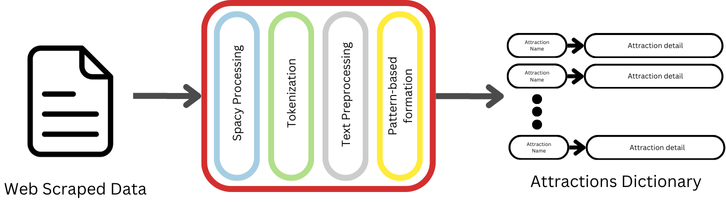
\includegraphics[width=1\linewidth]{NLP-Processor.png}
        \caption{NLP Processor}
        \label{fig:nlp-processor}
    \end{figure}


\section{Methodology and Models}

    \subsection{Initial Approach}

        Initially, we utilized various models to do two distinct tasks: question answering and text-to-text generation. The models employed for each task are enumerated below:

        \subsubsection{Question Answering Models}
            For the question answering task, we employed the following models:
            \begin{itemize}
                \item BERT
                \item RoBERTa
                \item DistilBERT
            \end{itemize}

            The models were employed to address inquiries pertaining to the context presented in the dataset. The main goal was to obtain important insights and precise replies from the processed scraped data. The specific questions asked to the models are:

            \begin{tcolorbox}[linewidth=1pt, innerleftmargin=15pt, innerrightmargin=15pt, innertopmargin=15pt, innerbottommargin=15pt]
                \begin{enumerate}
                    \item What is the name of the attraction?
                    \item What is the location of the attraction?
                    \item Describe the attraction in detail.
                    \item What type of attraction is it? (e.g., historical, natural, amusement, beach)
                \end{enumerate}
            \end{tcolorbox}

        \subsubsection{Text-to-Text Generation Models}
            For the text-to-text generation task, specifically summarization, we utilized the following models:
            \begin{itemize}
                \item T5
                \item Llama-3
            \end{itemize}

            The models were optimized to generate precise and concise summaries, compressing the text while preserving its significance and relevance. This approach was crucial for producing succinct descriptions of tourist destinations from extensive web-scraped data.

            Our objective was to improve the comprehension and utility of the gathered data by utilizing these models, hence increasing its accessibility and providing users with more interesting insights.
        {\\}
         \subsubsection{Itenary generation Model}
            For this task, we utilized Ollama, specifically employing the Llama 3.1 model. The Ollama model was instrumental in generating detailed and personalized travel itineraries by processing the cleaned text, which had previously undergone NLP processing and summarization through T5 and Llama.
{\\}
    \subsection{Data Collection and Preprocessing}

        The data for fine-tuning the models was sourced from various online travel platforms, focusing on popular tourist destinations, including detailed descriptions, locations, types of attractions, and user reviews. To ensure high-quality input, the data was pre-processed by performing several steps:

        \begin{itemize}
            \item \textbf{Tokenization:} Text data was tokenized using the respective model tokenizers.
            \item \textbf{Cleaning:} Non-ASCII characters, HTML tags, and extra whitespace were removed.
            \item \textbf{Normalization:} Text was converted to lowercase, and punctuation was standardized.
            \item \textbf{Splitting:} The data was divided into training and evaluation sets with an 80:20 ratio.
        \end{itemize}

        This comprehensive preprocessing ensured that the models received noise-free and relevant data, enhancing the accuracy and relevance of the generated travel itineraries.


        We created two datasets for fine-tuning, each with a different purpose:

        \begin{enumerate}
            \item \textbf{Summarization Dataset}: The dataset was utilized to refine the Llama-3 and Flan-T5 models. The system was comprised of two components: context and summary. The context pertained to the data obtained by web scraping, while the summary was a concise translation of the text that was both grammatically correct and concise.\\


            \item \textbf{Question-Answering Dataset}: The dataset was utilized to refine Question-Answering Models, specifically BERT, DistilBERT, and RoBERTa. The document has six questions as specified in the annexure. The dataset was utilized to get significant insights from the processed scraped data.
        \end{enumerate}

    \subsection{Question Answering Model Configurations}

        \subsubsection{BERT}

            BERT, developed by Google, was fine-tuned using the following configurations:
            \begin{itemize}
                \item Model: \texttt{bert-base-uncased}
                \item Tokenizer: \texttt{BertTokenizer}
                \item Training epochs: 3
                \item Learning rate: 5e-5
                \item Batch size: 8
            \end{itemize}

        \subsubsection{RoBERTa}

            RoBERTa, an optimized version of BERT, was used to enhance the contextual understanding of travel-related queries. The following configurations were used:
            \begin{itemize}
                \item Model: \texttt{deepset/roberta-base-squad2}
                \item Tokenizer: \texttt{AutoTokenizer}
                \item Training epochs: 3
                \item Learning rate: 2e-5
                \item Batch size: 8
            \end{itemize}

        \subsubsection{DistilBERT}

            DistilBERT, a distilled version of BERT, was fine-tuned with reduced computational requirements:
            \begin{itemize}
                \item Model: \texttt{distilbert-base-uncased}
                \item Tokenizer: \texttt{DistilBertTokenizer}
                \item Training epochs: 3
                \item Learning rate: 5e-5
                \item Batch size: 8
            \end{itemize}

    \subsection{Text2Text Generation Model Configurations}

        \subsubsection{T5}

            T5, also from Google, was treated as a text-to-text problem and fine-tuned with the following settings:
            \begin{itemize}
                \item Model: \texttt{google/flan-t5-small}
                \item Tokenizer: \texttt{AutoTokenizer}
                \item Training epochs: 10
                \item Learning rate: 2e-5
                \item Batch size: 16
            \end{itemize}

\begin{tcolorbox}[linewidth=1pt, innerleftmargin=15pt, innerrightmargin=15pt, innertopmargin=15pt, innerbottommargin=15pt]
\begin{lstlisting}
\small
\begin{verbatim}
Training_args = Seq2SeqTrainingArguments(
    evaluation_strategy="epoch",
    learning_rate=2e-5,
    per_device_train_batch_size=10,
    per_device_eval_batch_size=10,
    weight_decay=0.01,
    save_total_limit=3,
    num_train_epochs=10
)
\end{verbatim}
\end{lstlisting}
\end{tcolorbox}

        \subsubsection{Llama}

            Llama, known for its large-scale language understanding capabilities, was fine-tuned using the Unsloth framework:
            \begin{itemize}
                \item Model: \texttt{unsloth/llama-3-8b-bnb-4bit}
                \item Tokenizer: \texttt{FastLanguageModel}
                \item Max steps: 30
                \item Learning rate: 2e-4
                \item Batch size: 16
                \item Use gradient checkpointing: \texttt{unsloth}
            \end{itemize}

\begin{tcolorbox}[linewidth=0.5pt, innerleftmargin=10pt, innerrightmargin=10pt, innertopmargin=10pt, innerbottommargin=10pt, fontupper=\footnotesize]
\begin{verbatim}
TrainingArguments(
    per_device_train_batch_size = 2,
    gradient_accumulation_steps = 4,
    warmup_steps = 5,
    max_steps = 30,
    learning_rate = 2e-4,
    fp16 = not torch.cuda.is_bf16_supported(),
    bf16 = torch.cuda.is_bf16_supported(),
    logging_steps = 1,
    optim = "adamw_8bit",
    weight_decay = 0.01,
    lr_scheduler_type = "linear",
    seed = 3407,
    output_dir = "outputs",
)
\end{verbatim}
\end{tcolorbox}

\section{Results and Evaluation}

    The training and evaluation losses for DistilBERT, RoBERTa, and BERT models were analyzed to assess their performance on the QA tasks. These losses are depicted in Figures \ref{fig:training-loss-qa} and \ref{fig:evalutation-loss-qa}, respectively.
    {\\}

    \begin{figure}
        \centering
        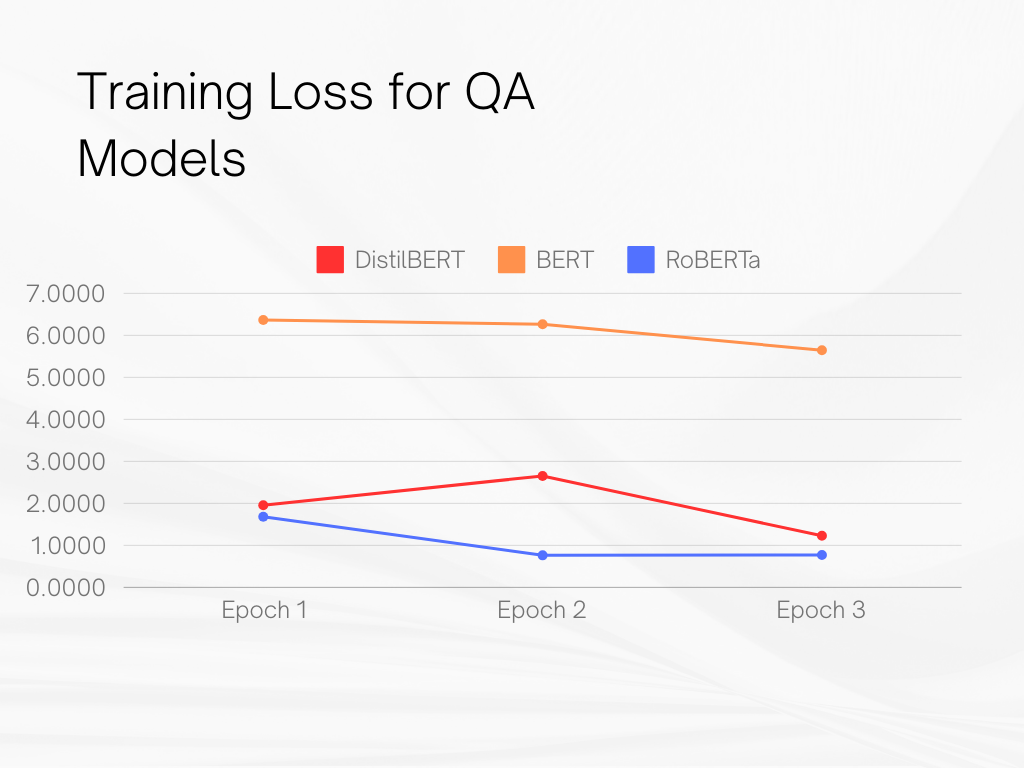
\includegraphics[width=1\linewidth]{Training-Loss.png}
        \caption{Training Loss For QA Models}
        \label{fig:training-loss-qa}
    \end{figure}

    \begin{figure}
        \centering
        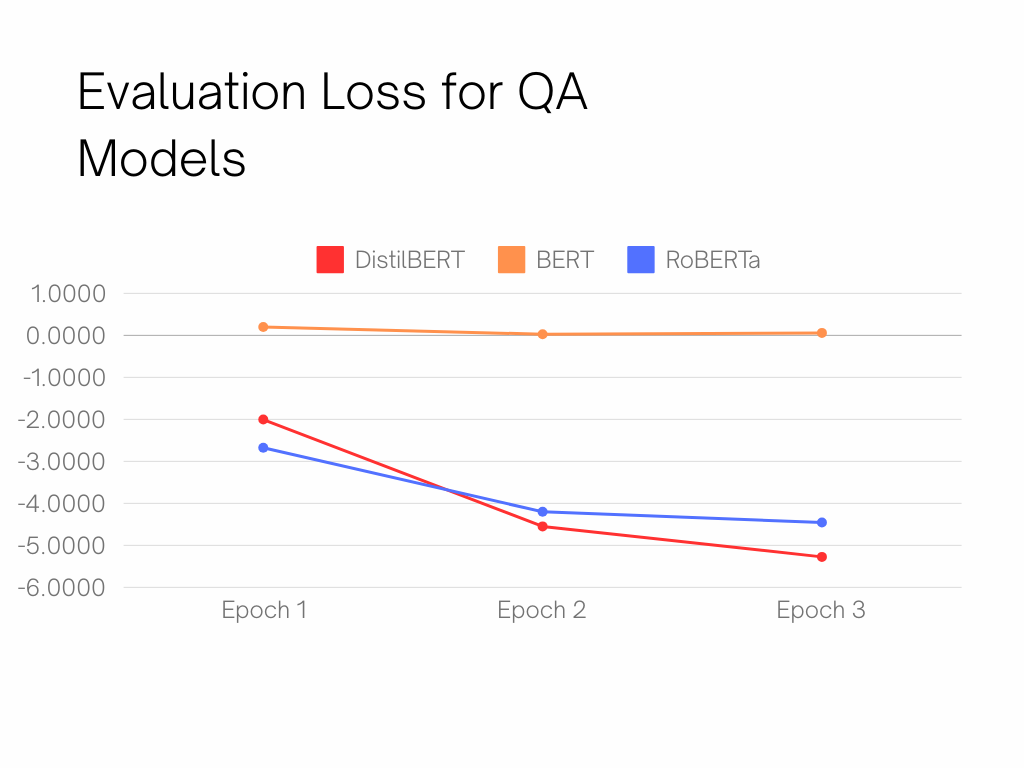
\includegraphics[width=1\linewidth]{Evaluation-Loss.png}
        \caption{Evaluation Loss For QA Models}
        \label{fig:evalutation-loss-qa}
    \end{figure}

    In Figure \ref{fig:training-loss-qa}, the training losses show a consistent decline across all models, indicating that the models are learning effectively during training. However, Figure \ref{fig:evalutation-loss-qa} reveals negative evaluation loss scores, pointing to potential issues in the evaluation phase. These negative scores suggest that the models may have struggled to capture context from the dataset, possibly due to limitations in the dataset itself or misalignment in the fine-tuning process.
    {\\}

    Additionally, the training process for Llama 3 - 8B was evaluated, as shown in Figure \ref{fig:llama-training-loss}. The training loss decreased over steps, demonstrating the model's ability to learn. Despite fluctuations, the overall trend suggests a learning curve that could benefit from further refinement or additional epochs to achieve better stability and convergence.

    \begin{figure}
        \centering
        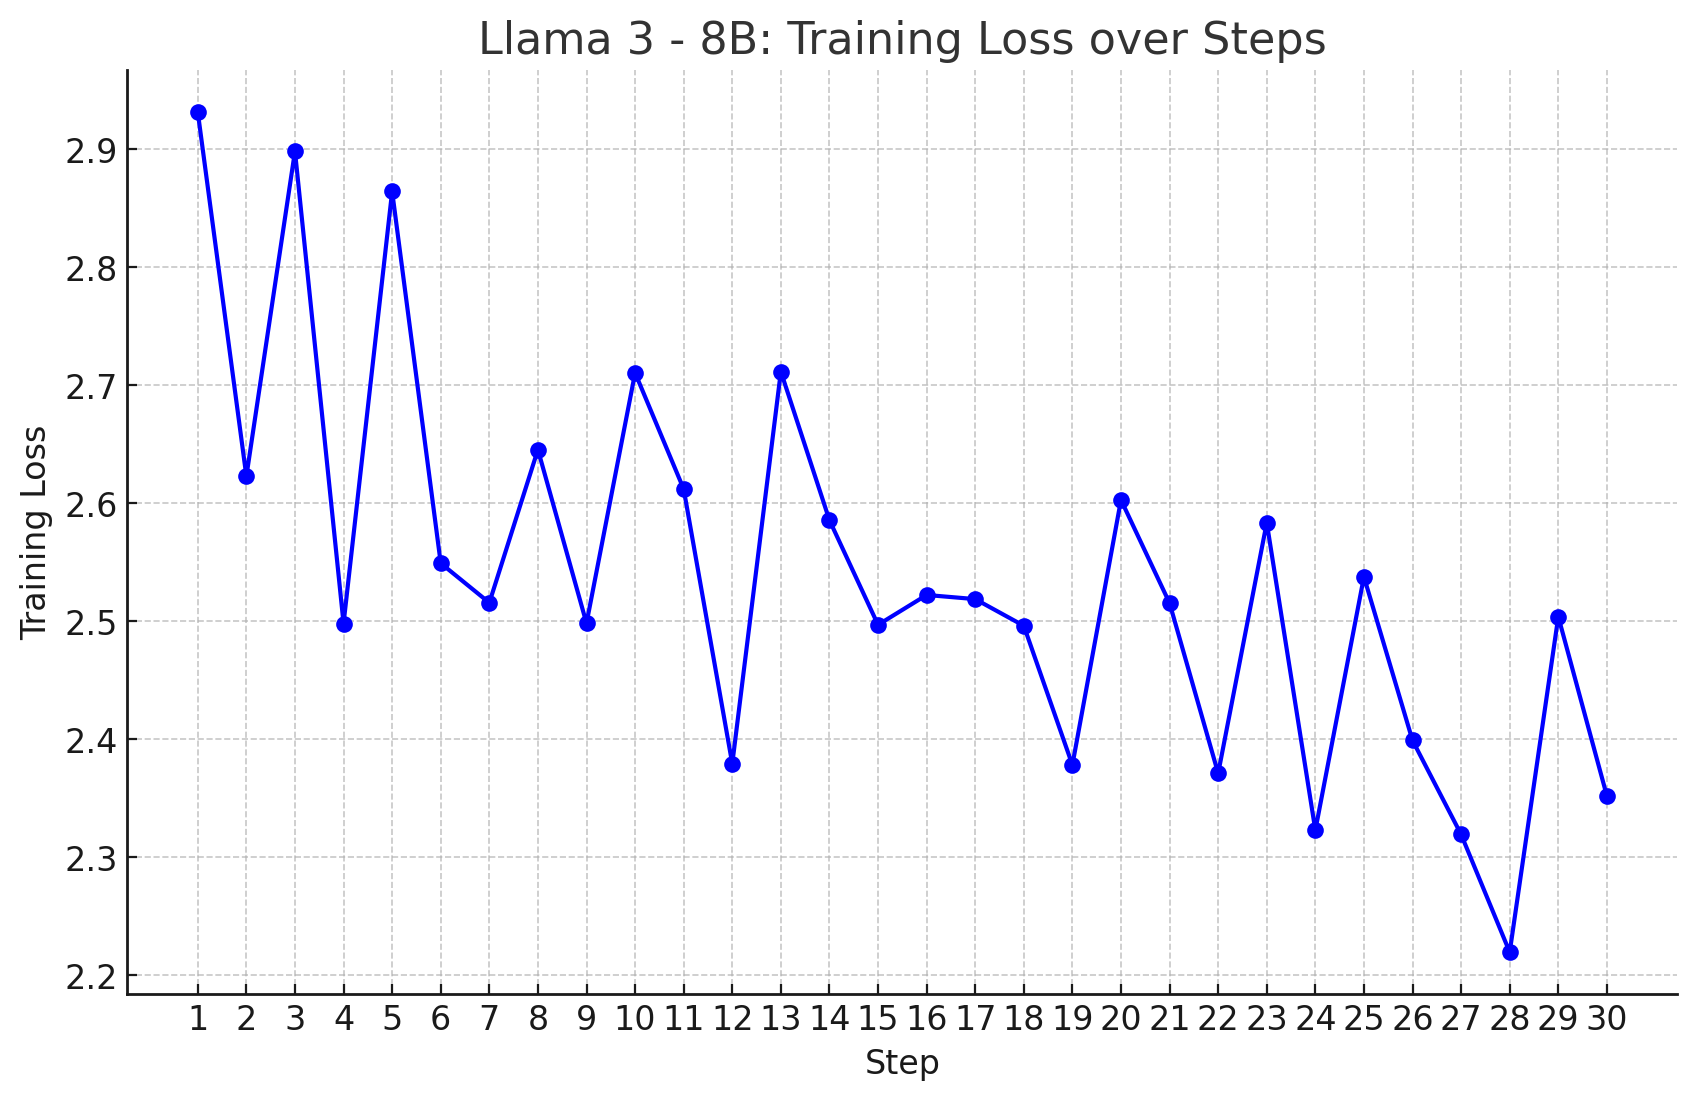
\includegraphics[width=1\linewidth]{Llama-Training-Loss.png}
        \caption{Llama Training Loss Over Steps}
        \label{fig:llama-training-loss}
    \end{figure}

    These results highlight the models' learning capabilities and the challenges faced during evaluation, offering insights for future improvements in model fine-tuning and dataset selection.


\section{Transformer Models and Pipeline Integration}

    \subsection{T5}

    We fine-tuned Google's FLAN T5 Transformer, available in our Hugging Face models repository, to compress sentences from NLP-scraped text. This approach effectively captured key points with impressive speed. However, we encountered several issues:

    \subsubsection{Issues Faced}
    \begin{itemize}
        \item \textbf{Short Sentences:} Generated text was often overly brief, leading to a fragmented narrative.
        \item \textbf{Punctuation Problems:} Inconsistent punctuation resulted in unclear descriptions.
        \item \textbf{Conciseness and Accuracy:} While quick, the summaries sometimes omitted important details and lacked precision.
    \end{itemize}

    These challenges indicated the need for a model that could produce well-structured, punctuated text while maintaining T5's speed and efficiency.

    \subsection{Llama}

    Our fine-tuned LLaMA model generated accurate descriptions with high precision. However, it posed significant challenges in processing time and computational resource demands.

    \subsubsection{Issues Faced}
    \begin{itemize}
        \item \textbf{Repetition of Sentences:} The model often repeated sentences, affecting coherence.
        \item \textbf{Punctuation Problems:} Descriptions frequently lacked proper punctuation, leading to unclear text.
        \item \textbf{Abrupt Endings:} Some outputs ended abruptly, resulting in incomplete descriptions.
    \end{itemize}

    We experimented with model parameters like text streamer output size, temperature values, and other hyperparameters to improve accuracy. However, these adjustments increased processing time significantly, creating a trade-off between accuracy and speed that limited the model's practicality for real-time applications.


    \subsection{Comparison of Sample Outputs: T5 vs. Llama}

        \begin{tcolorbox}[linewidth=1pt, innerleftmargin=15pt, innerrightmargin=15pt, innertopmargin=15pt, innerbottommargin=15pt]
            \textbf{Context:} \\

            Cubbon Park Sarangib for Pixabay Situated over a sprawling 300 acres of land the park was constructed by Richard Sankey This massive green park along with lawns deserves a special mention Offering statues of famous personalities the park is one among the popular places to visit in Bangalore with friends Location Kasturba Road Behind High Court of Karnataka Ambedkar Veedhi Sampangi Rama Nagara BangaloreTimings Open on all daysEntry Fee No entry fee Suggested Read Resorts Near Bangalore
        \end{tcolorbox}


        \begin{tcolorbox}[linewidth=1pt, innerleftmargin=15pt, innerrightmargin=15pt, innertopmargin=15pt, innerbottommargin=15pt]
            \textbf{T5 Output:} \\

            Cubbon Park, a sprawling 300 acres of land, is a popular place to visit in Bangalore with friends. Offering statues of famous personalities, it is a popular place to visit with friends.
        \end{tcolorbox}

        \begin{tcolorbox}[linewidth=1pt, innerleftmargin=15pt, innerrightmargin=15pt, innertopmargin=15pt, innerbottommargin=15pt]
            \textbf{Llama3 Output:} \\

            The park was constructed by Richard Sankey. This massive green park, along with lawns, deserves a special mention. Offering statues of famous personalities, the park is one among the popular places to visit in Bangalore with friends. Location: Kasturba Road, Behind High Court of Karnataka.
        \end{tcolorbox}

    \subsection{Understanding the Advantages and Disadvantages of LLaMA and T5 Models}

        After assessing the advantages and disadvantages of both the LLaMA and T5 large language models, we developed a new pipeline designed to leverage the strengths of both models. In this pipeline, we used the T5 Transformer to generate concise descriptions from the web scrape for each attraction. These brief summaries were then passed to the LLaMA model for elaboration. This approach aimed to combine the speed of T5 with the detail-oriented capabilities of LLaMA.\\

        \subsubsection{{\textbf{Pipeline Implementation}}}
            \begin{itemize}
                \item \textbf{Concise Descriptions with T5:} The T5 Transformer efficiently generated short, informative summaries of the web-scraped text, capturing the key points of each attraction with impressive speed.
                \item \textbf{Elaboration with LLaMA:} These summaries were subsequently elaborated upon by the LLaMA model to provide detailed and comprehensive descriptions.
            \end{itemize}


            Using LLaMA in this manner significantly reduced the time required compared to using it directly on the raw web-scraped text.

            \begin{figure}
                \centering
                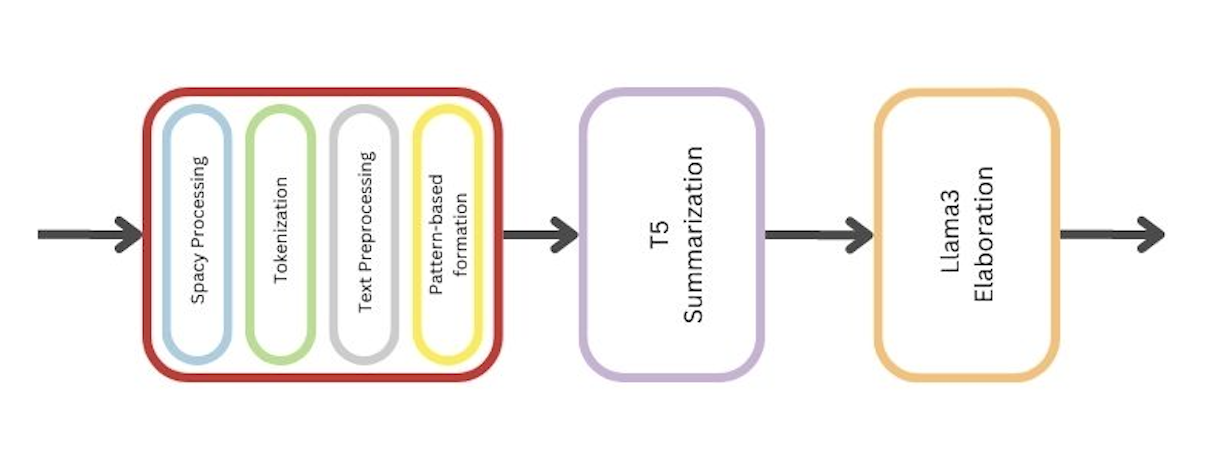
\includegraphics[width=1\linewidth]{Pipeline.png}
                \caption{Pipeline Overview}
                \label{fig:pipeline}
            \end{figure}

        \subsubsection{\textbf{Pipeline Results}}

            To illustrate the effectiveness of our pipeline, we present a sample context along with the outputs generated by T5 and LLaMA models.

            \begin{tcolorbox}[linewidth=1pt, innerleftmargin=15pt, innerrightmargin=15pt, innertopmargin=15pt, innerbottommargin=15pt]
                \textbf{Context:} \\

                \small
                Sahastradhara If you are looking for the best place in Dehradun to visit in June you can't miss the magnificent waterfalls of Sahastradhara. The waterfall is the perfect emblem of its name as Sahastradhara means spring. Not only the waterfalls but you can also visit the steppe farming land and caves at this place which creates a perfect panoramic view for entertaining the tourists. Along with enjoying the natural beauty of this place you can also take a fun ride in the air through ropeways. Once you travel by ropeway the stunning view of the mountains and valleys will enthrall you completely. The water of Sahastradhara falls is and that’s why it has lots of medicinal benefits. Though you can visit this place throughout the year, monsoon is the best time to visit Sahastradhara at its best. Where 11km from Dehradun near Robber's CaveTimings 8 am to 7 pm Entry Fee Free Suggested Read 20 Cafes In Dehradun That Are Too Awesome To Resist
            \end{tcolorbox}


            The T5 transformer model subsequently processes the context. The T5 model is specifically engineered to produce concise overviews from the provided text input, extracting the most important details. The following is the output that concisely captures the main points of the provided context:

            \begin{tcolorbox}[linewidth=1pt, innerleftmargin=15pt, innerrightmargin=15pt, innertopmargin=15pt, innerbottommargin=15pt]
                \textbf{T5 Output:} \\

                \small
                Sahastradhara is known for its magnificent waterfalls, steppe farming land, and caves. The waterfall is a perfect emblem of its name. It offers a panoramic view of the mountains and valleys. The water of Sahastradhara falls is renowned for its medicinal benefits. Visit Monsoon from Dehradun from 8 am to 7 pm. Entry fee is free. Read 20 Cafes In Dehradun That Are Too Awesome To Resist. The waterfall is a great place to visit in June.. Sahradhara's beautiful, and
            \end{tcolorbox}

            Following that, the LLaMA-3 model is provided with the concise summary produced by the T5 transformer for further elaboration and appropriate punctuation. The summary is further elaborated upon by the LLaMA-3 model, which guarantees that the text is well-organized and comprehensible.

            \begin{tcolorbox}[linewidth=1pt, innerleftmargin=15pt, innerrightmargin=15pt, innertopmargin=15pt, innerbottommargin=15pt]
                \textbf{Llama Output:} \\

                \small
                It is one of Uttarakhand's most popular tourist attractions. Located at a distance of 16 km from the city, it is surrounded by lush greenery and has a waterfall that falls from a height of more than 200 feet. There is also a cave in the area that is believed to have medicinal properties. You can visit this place with your family and friends and enjoy the beauty of nature.
            \end{tcolorbox}

        \subsubsection{\textbf{Issues Faced}}
            Despite the improvements, we encountered several challenges:
            \begin{itemize}
                \item \textbf{Processing Time:} LLaMA still required a significant amount of time and computational overhead for elaborating on each attraction. Each page, containing 10 attractions, took approximately 1.5 to 2 minutes to process.
                \item \textbf{Resource Intensity:} The detailed elaboration by LLaMA, while more efficient than direct processing, still demanded considerable computational resources, impacting the overall efficiency of the pipeline.
            \end{itemize}

    \subsection{Building a successful pipeline for our use-case}

        The final objective of our project was to generate a personalized itinerary for users based on the number of days they planned to travel. Initially, we used our trained version of the LLaMA model for this task but quickly realized that it posed significant challenges in terms of efficiency and processing time. Consequently, we decided to utilize the Ollama model for the final itinerary generation.

        \subsubsection{Pipeline Overview}
            \begin{itemize}
                \item \textbf{NLP Processing:} The web page containing attraction details is first subjected to NLP processing to clean and organize the data. This processed data is divided into chunks representing individual attractions.
                \item \textbf{Summarization with T5:} These chunks are then passed to the T5 Transformer, which performs the summarization task. The T5 model generates concise sentences summarizing each attraction, and these summaries are stored in a dictionary format for easy retrieval.
                \item \textbf{Itinerary Generation with Ollama:} Using the user-provided input regarding the number of days for their trip, the Ollama model generates a detailed itinerary using the summarized attractions produced by T5 transformer
            \end{itemize}

        \subsubsection{Challenges and Observations}
            \begin{itemize}
                \item \textbf{Efficiency:} The LLaMA model, while accurate, proved to be inefficient for real-time itinerary generation due to its high processing time. Each page with 10 attractions took approximately 1.5 to 2 minutes, which was not feasible for a user-friendly application.
                \item \textbf{Improved Workflow with Ollama:} By integrating Ollama into the pipeline, we significantly reduced the processing time and improved the overall efficiency. The T5 model's summarization capabilities combined with Ollama's itinerary planning provided a balanced solution, offering both speed and accuracy.
            \end{itemize}

            \begin{figure}
                \centering
                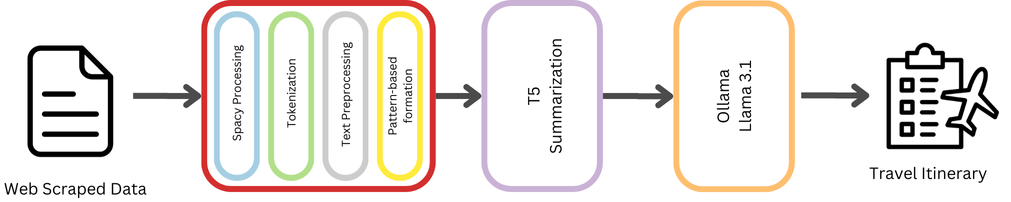
\includegraphics[width=1\linewidth]{Final-Pipeline.png}
                \caption{Final Pipeline Implentation}
                \label{fig:final-pipeline}
            \end{figure}

    \subsection{Using Ollama for itinerary generation}

        Ollama is a platform that is capable of building and deploying machine learning models and can support a wide variety of architectures, such as transformers, CNNs, RNNs, ensemble models, and GNNs. It enhances the efficacy and effectiveness of a diverse array of machine learning tasks by simplifying workflows from preprocessing to deployment. Llama 3.1, Gemma 2, and other models are among the models it supports.

        We are utilizing Ollama to generate itineraries and are currently operating the Llama 3.1 model. The NLP processor's list of attractions is incorporated into the prompt for Ollama to assist in the generation of the itinerary, using the processed text that has been obtained after conducting NLP on the scraped text (as previously detailed). More than 4 minutes are required to generate the itinerary wholly without providing data using Ollama in the absence of the attractions list. The itinerary is generated in approximately 2 to 2.5 minutes after the data has been incorporated.

        \begin{tcolorbox}[colframe=black!75!white, colback=white!90!black, title=Ollama Prompt to generate itinerary]
        Generate a detailed itinerary for me for a \{days\} day trip and here are the suggested places I would like to cover:

        1: Attraction 1 \\
        Attraction Description\\

        2: Attraction 2 \\
        Attraction Description\\

        3: Attraction 3 \\
        Attraction Description\\

        % Repeat for each attraction

        and so on.
        \end{tcolorbox}


    \subsection{Incorporating User Preferences}

        The investigation of user preferences in itinerary planning is a primary objective of our research, focusing on historical, amusement, and natural attractions. Before planning, users provided assessments of these attributes, which were incorporated into the prompt used by Ollama to generate itineraries. This integration led to more personalized and satisfactory travel plans.

        This pipeline successfully meets the project's goal of generating customized itineraries, showcasing the effective combination of T5 and Ollama in handling large-scale data and delivering user-centric solutions.

\begin{tcolorbox}[colframe=black!75!white, colback=white!90!black, title=Sample One-Day Itinerary with User Preferences]
Day 1: Historical Exploration
\begin{itemize}
    \item \textbf{Morning:} Visit India Gate (9:00 am - 10:30 am)
    \begin{itemize}
        \item \textit{Description:} Start your day by paying respects at the iconic India Gate monument.
    \end{itemize}
    \item \textbf{Afternoon:} Visit Lotus Temple (11:00 am - 12:30 pm)
    \begin{itemize}
        \item \textit{Description:} Explore the beautiful and serene Lotus Temple, a perfect place for history buffs.
    \end{itemize}
\end{itemize}
\end{tcolorbox}

\begin{tcolorbox}[colframe=black!75!white, colback=white!90!black, title=Sample One-Day Itinerary without User Preferences]
Day 1: India Gate, Lotus Temple, and Akshardham Temple
\begin{itemize}
    \item \textbf{Morning:} Start your day by visiting India Gate, a monument commemorating Indian soldiers from World War I.
    \item \textbf{Next:} Head to Lotus Temple, a must-visit for history buffs and spiritual seekers.
    \item \textbf{Afternoon:} After lunch, visit Akshardham Temple, catching the stunning evening lighting.
\end{itemize}
\end{tcolorbox}

The first itinerary prioritizes user preferences, while the second focuses on covering attractions listed in the prompt. The samples illustrate how user input shapes the itinerary, with the first being a longer journey. In later interviews, participants were asked whether they preferred faster itinerary generation without user preferences or valued personalized itineraries despite longer processing times.


\section{Discussion}

    \subsection{Question Answering Models}

        The models' poor evaluation scores reveal significant challenges in accurately predicting relevant details from attraction descriptions. Despite extensive preprocessing and fine-tuning, the models struggled with understanding the input data, leading to imprecise responses. The complexity and diversity of the data likely contributed to low or negative scores, emphasizing the need for further model refinement or alternative approaches to enhance prediction accuracy.

    \subsection{Text-to-Text Generation Model Inferences}

    During our evaluation of text-to-text generation models, T5 and LLaMA-3, several key observations were made:

    \begin{enumerate}
        \item \textbf{Speed and Loading Time:} T5 exhibited faster processing and shorter loading times compared to LLaMA-3, making it suitable for real-time applications.

        \item \textbf{Handling of Content:} T5 sometimes omitted the attraction's name in summaries, while LLaMA-3 consistently included it, providing a clearer and more organized output.

        \item \textbf{Grammatical Accuracy:} T5 maintained better grammatical accuracy, resulting in more refined and readable summaries.

        \item \textbf{Combinations and Results:} We tested various combinations, such as T5-LLaMA in series and LLaMA-LLaMA in series, along with individual use of T5 and LLaMA with BERT for extracting details. The T5-LLaMA combination was the most effective, balancing speed and detail.

        \item \textbf{Itinerary Generation:} Although LLaMA's long processing time posed challenges, we employed Ollama, based on LLaMA 3.1, to meet itinerary generation requirements effectively.
    \end{enumerate}

    These findings highlight the strengths and weaknesses of T5 and LLaMA-3 in content summarization. T5's speed and grammatical accuracy make it ideal for rapid tasks, while LLaMA-3 excels in structured content delivery. Balancing these factors is crucial when selecting models for real-world applications.


\section{Conclusion}

    The goal of this research was to identify the best combination of LLMs for generating and fine-tuning itineraries. Initially, we trained question-answering models to extract details from attraction descriptions, but they underperformed. We then focused on text-to-text generation models, specifically LLaMA-3 and T5, for summarization.

    Our experiments showed that while T5 is faster at summarization, it is sometimes less detailed than LLaMA-3. Given our priority on speed, we selected T5 for summarization, pairing it with LLaMA for its detailed output. Ollama, based on LLaMA 3.1, was used for efficient itinerary generation.

    We also investigated user preferences in itinerary planning, integrating them into Ollama's prompt for more personalized and satisfactory travel plans.

    In conclusion, the combination of T5 and LLaMA provided a balanced approach, ensuring both efficiency and comprehensiveness, while incorporating user preferences significantly enhanced personalization in travel itineraries.


    \subsection{Future Work}

        Future work will aim to optimize model performance and efficiency, focusing on:
        \begin{itemize}
            \item Exploring additional NLP models and architectures for further improvements.
            \item Enhancing data collection and preprocessing to improve training data quality and diversity.
            \item Integrating user feedback to refine and personalize itinerary recommendations.
            \item Expanding the models' application to other travel industry domains, such as real-time assistance and dynamic itinerary adjustments.
        \end{itemize}


    \subsection{Potential Applications}

        This study demonstrates the potential of advanced NLP techniques in transforming travel planning. The successful implementation in Roamify shows these models can generate accurate and personalized itineraries. Potential applications include:

        \begin{itemize}
            \item Personalized travel planning services tailored to individual preferences.
            \item Real-time travel assistance tools offering dynamic recommendations.
            \item Enhanced customer support systems providing quick, accurate responses.
        \end{itemize}

        In conclusion, integrating NLP models into tools like Roamify boosts the efficiency and personalization of travel experiences. Continued research will further enhance AI's role in delivering more intuitive and responsive travel planning solutions.


\section{User Survey and Interview Analysis}

    \subsection{Survey Methodology}
        To understand potential users' travel planning behaviors and preferences for Roamify, we conducted a comprehensive survey across various demographic groups. The survey included multiple-choice and open-ended questions to capture insights into travel habits, challenges in planning, and expectations from a travel tool. The survey and interview responses are available here: \href{https://drive.google.com/drive/folders/1mKPTXZ7n7ZFmMEK6QBOKU0op3mf8hCta?usp=sharing}{\textbf{Survey Interviews}}.


    \subsection{Survey Results and Analysis}
        The survey received responses from a substantial number of participants, covering a diverse range of age groups and travel frequencies.
        \\

        \textbf{Key Insights from Surveys:}

        \begin{itemize}
            \item \textbf{Demographic Breakdown}: Most respondents were young adults (19-25 years) and adults (26-64 years), indicating travel planning is significant among working professionals and young individuals (Figure \ref{fig:demographic-distribution}).
            \begin{figure}
                \centering
                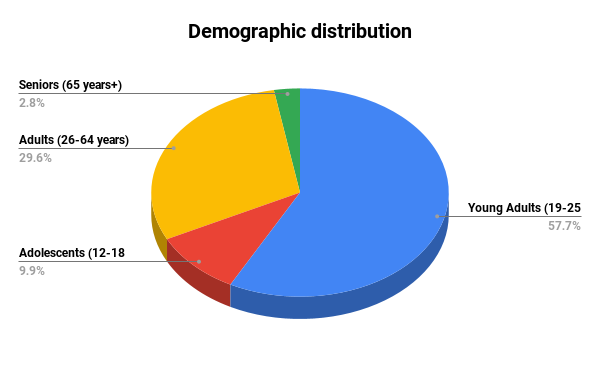
\includegraphics[width=0.75\linewidth]{Demographic-distribution.png}
                \caption{Demographic Distribution}
                \label{fig:demographic-distribution}
            \end{figure}
            \item \textbf{Travel Frequency}: Most respondents travel once every 6 months or annually, preferring occasional travel due to work and life commitments (Figure \ref{fig:travel-frequency}).
            \begin{figure}
                \centering
                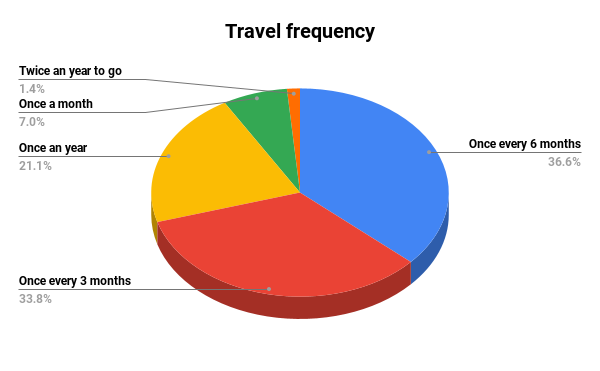
\includegraphics[width=0.75\linewidth]{Travel-frequency.png}
                \caption{Travel Frequency}
                \label{fig:travel-frequency}
            \end{figure}
            \item \textbf{Types of Travel}: Casual, entertainment, and work travel are the most common, highlighting the importance of leisure and professional commitments in travel plans (Figure \ref{fig:types-of-travel}).
            \begin{figure}
                \centering
                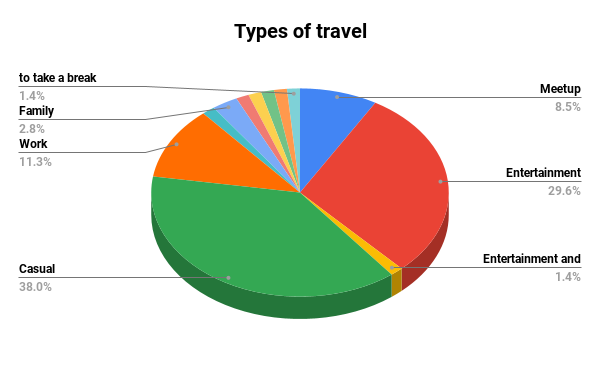
\includegraphics[width=0.75\linewidth]{Types-of-travel.png}
                \caption{Types of Travel}
                \label{fig:types-of-travel}
            \end{figure}
            \item \textbf{Itinerary Planning}: Online travel websites and YouTube are primary sources, showing a shift towards digital platforms for travel information (Figure \ref{fig:itenary-decision}).
            \begin{figure}
                \centering
                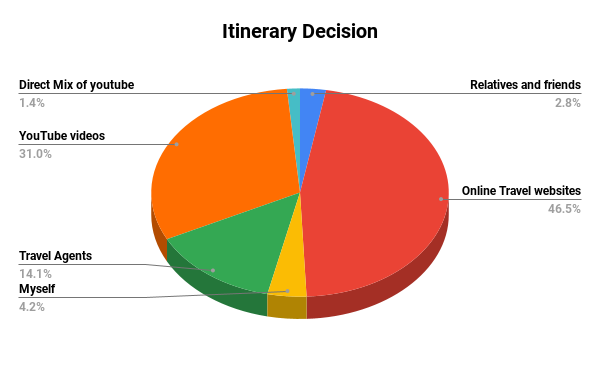
\includegraphics[width=0.75\linewidth]{Itinerary-Decision.png}
                \caption{Itinerary Decision}
                \label{fig:itenary-decision}
            \end{figure}
            \item \textbf{Customization Preferences}: A significant majority prefer customized itineraries, emphasizing the demand for personalized travel tools (Figure \ref{fig:customization-preferences}).
            \begin{figure}
                \centering
                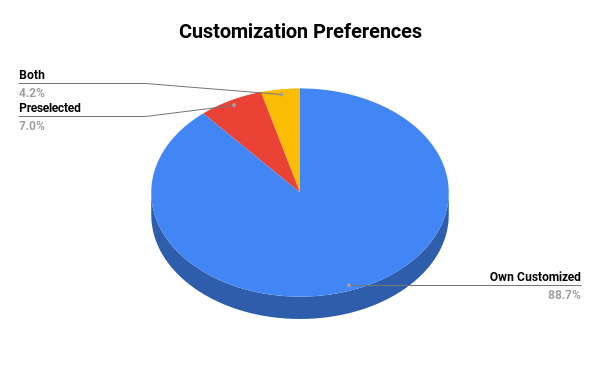
\includegraphics[width=0.75\linewidth]{Customization-Preferences.png}
                \caption{Customization Preferences}
                \label{fig:customization-preferences}
            \end{figure}
            \item \textbf{Satisfaction with Travel Agencies}: Satisfaction levels vary, with moderate satisfaction indicating areas for improvement in travel agency services (Figure \ref{fig:satisfaction-with-travel-agencies}).
            \begin{figure}
                \centering
                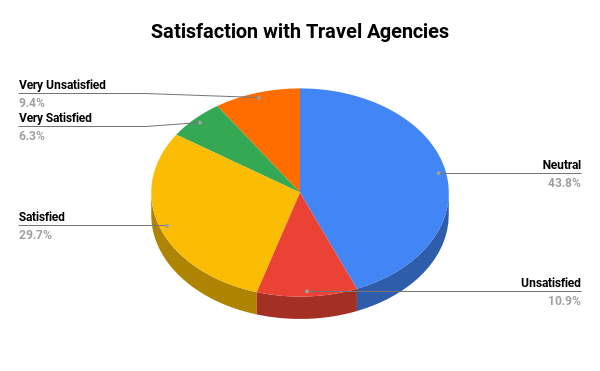
\includegraphics[width=0.75\linewidth]{Satisfaction-with-Travel-Agencies.png}
                \caption{Satisfaction with Travel Agencies}
                \label{fig:satisfaction-with-travel-agencies}
            \end{figure}
            \item \textbf{Challenges in Planning}: Key challenges include information overload, coordination difficulties, and a lack of personalized recommendations, making planning time-consuming and stressful (Figures \ref{fig:custom-itinerary-build-time}).
        \end{itemize}
            \begin{figure}
                \centering
                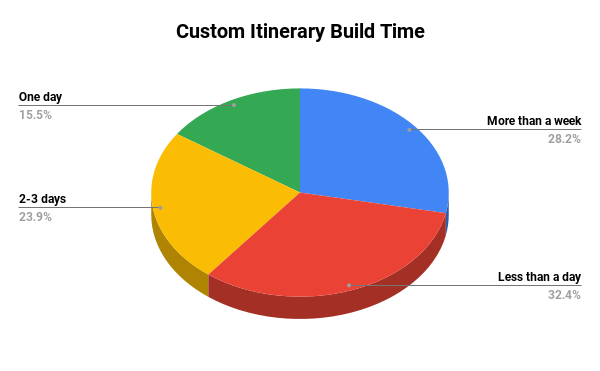
\includegraphics[width=0.75\linewidth]{Custom-Itinerary-Build-Time.png}
                \caption{Custom Itinerary Build Time}
                \label{fig:custom-itinerary-build-time}
            \end{figure}
            % \begin{figure}
            %     \centering
            %     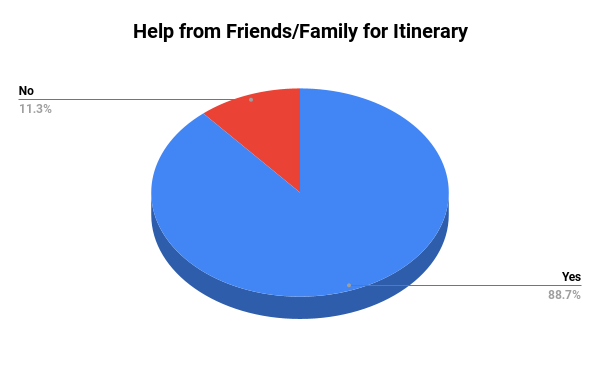
\includegraphics[width=0.75\linewidth]{Help-from-Friends-Family-for-Itinerary.png}
            %     \caption{Help from Friends & Family for Itinerary}
            %     \label{fig:help-from-friends-family-for-itinerary}
            % \end{figure}

    \subsection{Interview Methodology and Findings}
        In addition to the survey, in-depth interviews were conducted to gain deeper insights into travel planning experiences, focusing on pain points and expectations from a travel planning tool.

        \textbf{Key Insights from Interviews:}
        \begin{itemize}
            \item \textbf{Frequency of Travel:} Interviewees typically travel 3-4 times a year, requiring flexible and comprehensive planning tools.
            \item \textbf{Planning Process:} Extensive research, price comparisons, and seeking recommendations from friends and family highlight the complexity and time-consuming nature of travel planning.
            \item \textbf{Challenges:} Common challenges include information overload, coordination issues, and the need for reliable, personalized recommendations.
            \item \textbf{Expectations from AI Tools:} Participants prefer AI tools that offer tailored recommendations, streamline booking, and provide real-time updates, integrating multiple information sources.
            \item \textbf{Personalization:} 60\% of interviewees emphasized the need for tools that adapt to their unique interests and preferences.
            \item \textbf{User Experience:} Demand is high for user-friendly interfaces with seamless platform integration, clear information, and robust customer support.
            \item \textbf{Age Group Preferences:} Generation X prefers offline travel agencies, while Millennials and Generation Z favor online agencies and AI-generated itineraries, considering factors like weather, budget, and intercity travel.
            \item \textbf{Waiting Time Concerns:} 80\% of interviewees stressed the importance of reducing waiting times for adopting AI tools in travel planning.
        \end{itemize}


    \subsection{Ongoing Implications}
        Survey and interview results show the need for Roamify, a comprehensive, individualized trip planning tool. Information overload, coordination challenges, and unpersonalised recommendations trouble users. Roamify can solve these problems and improve travel planning by using AI to provide customized itineraries, real-time updates, and an easy-to-use UI. Roamify will adapt to modern travelers' demands using these findings.


\newpage

\begin{thebibliography}{1}

    \bibitem{IEEEhowto:kopka}
        @article{article,
        author = {Filho, Angelo and Morabito, Reinaldo},
        year = {2023},
        month = {11},
        pages = {122437},
        title = {An effective approach for bi-objective multi-period touristic itinerary planning},
        volume = {240},
        journal = {Expert Systems with Applications},
        doi = {10.1016/j.eswa.2023.122437}
        }

    \bibitem{IEEEhowto:openai}
        OpenAI. (2023). "ChatGPT Release Notes." Retrieved from \url{https://help.openai.com/en/articles/6825453-chatgpt-release-notes}.

    \bibitem{IEEEhowto:econsultancy}
        Econsultancy. (2023). "Travel: How OTAs are adding generative AI to test the future of trip planning." Retrieved from \url{https://econsultancy.com/travel-ota-generative-ai/}.

    \bibitem{IEEEhowto:srdvtechnologies}
        SRDV Technologies. (2023). "Major Challenges Faced by Online Travel Agencies." Retrieved from \url{https://www.srdvtechnologies.com/blog/major-challenges-faced-by-online-travel-agencies}.

    \bibitem{ip2location}
        IP2Location, \emph{IP2Location IATA ICAO CSV}, \href{https://github.com/ip2location/ip2location-iata-icao/blob/master/iata-icao.csv}{https://github.com/ip2location/ip2location-iata-icao/blob/master/iata-icao.csv}.

    \bibitem{transformers}
        Hugging Face, \emph{Transformers Issue 27985 (with tracking parameters)}, \href{https://github.com/huggingface/transformers/issues/27985}{https://github.com/huggingface/transformers/issues/27985}.

    \bibitem{stackoverflow}
        Stack Overflow. Retrieved from \url{https://stackoverflow.com}.

    \bibitem{metawebsite}
        Meta. Retrieved from \url{https://about.meta.com}.

    \bibitem{youtube}
        YouTube, \emph{For training Llama Model using QLora and PEfT}, \href{https://www.youtube.com/watch?v=Vg3dS-NLUT4}{https://www.youtube.com/watch?v=Vg3dS-NLUT4}.

    \bibitem{llama}
        GitHub, \emph{Llama GitHub repository}, \href{https://github.com/facebookresearch/llama.git}{https://github.com/facebookresearch/llama.git}.

    \bibitem{spaCy}
        Explosion. (2023). "spaCy: Industrial-strength Natural Language Processing in Python." Retrieved from \url{https://spacy.io}.

    \bibitem{t5paper}
        Raffel, Colin, et al. "Exploring the limits of transfer learning with a unified text-to-text transformer." \emph{Journal of Machine Learning Research} 21.140 (2020): 1-67.

    \bibitem{bertpaper}
        Devlin, Jacob, et al. "BERT: Pre-training of Deep Bidirectional Transformers for Language Understanding." \emph{arXiv preprint arXiv:1810.04805} (2018).

    \bibitem{roberapaper}
        Liu, Yinhan, et al. "RoBERTa: A Robustly Optimized BERT Pretraining Approach." \emph{arXiv preprint arXiv:1907.11692} (2019).

    \bibitem{distilbertpaper}
        Sanh, Victor, et al. "DistilBERT, a distilled version of BERT: smaller, faster, cheaper and lighter." \emph{arXiv preprint arXiv:1910.01108} (2019).

    \bibitem{llamapaper}
        Touvron, Hugo, et al. "LLaMA: Open and Efficient Foundation Language Models." \emph{arXiv preprint arXiv:2302.13971} (2023).

    \bibitem{huggingface}
        Hugging Face. (2023). "Transformers: State-of-the-art Machine Learning for Pytorch, TensorFlow, and JAX." Retrieved from \url{https://github.com/huggingface/transformers}.

    \bibitem{nltk}
        Bird, Steven, Edward Loper, and Ewan Klein. "Natural language processing with Python: analyzing text with the natural language toolkit." \emph{"O'Reilly Media, Inc."} (2009).

    \bibitem{unsloth}
        Unsloth, \emph{Unsloth: An Efficient Library for Training Large Language Models}, \href{https://github.com/unsloth/unsloth}{https://github.com/unsloth/unsloth}.

    \bibitem{webscraping}
        Mitrevski, Marko. "Python Web Scraping: Hands-On Data Scraping and Crawling Using Pyspider, Splash, and Selenium." \emph{"Packt Publishing Ltd."} (2020).

    \bibitem{pythonselenium}
        SeleniumHQ. (2023). "Selenium WebDriver." Retrieved from \url{https://www.selenium.dev}.

    \bibitem{flant5}
        Heidloff, Niklas. (2023). "Fine-Tuning FLAN-T5." Retrieved from \url{https://heidloff.net/article/fine-tuning-flan-t5/}.

    \bibitem{flant5dc}
        DataCamp. (2023). "FLAN-T5 Tutorial." Retrieved from \url{https://www.datacamp.com/tutorial/flan-t5-tutorial}.

    \bibitem{flant5yt}
        YouTube. (2023). "FLAN-T5 Tutorial." Retrieved from \url{https://www.youtube.com/watch?v=PyRbP9d27sk}.

    \bibitem{llama3a}
        GitHub. (2023). "Unsloth: Efficient Library for Training Large Language Models." Retrieved from \url{https://github.com/unslothai/unsloth}.

    \bibitem{llama3b}
        Hugging Face Blog. (2023). "Fine-Tuning LLaMA-3 with Unsloth." Retrieved from \url{https://huggingface.co/blog/mlabonne/sft-llama3}.

    \bibitem{simpletransformers1}
        Towards Data Science. (2023). "Simple Transformers: Introducing the Easiest BERT, RoBERTa, XLNet, and XLM Library." Retrieved from \url{https://towardsdatascience.com/simple-transformers-introducing-the-easiest-bert-roberta}.
        % https://towardsdatascience.com/simple-transformers-introducing-the-easiest-bert-roberta-xlnet-and-xlm-library-58bf8c59b2a3

    \bibitem{simpletransformers2}
        YouTube. (2023). "Simple Transformers Tutorial." Retrieved from \url{https://www.youtube.com/watch?v=3XiJrn_8F9Q&t=1058s}.

\end{thebibliography}

\newpage

\appendix

\section{User Survey}
    To understand the travel planning behaviors and preferences of potential users for Roamify, we conducted a comprehensive survey. Below are the survey questions and the options provided for multiple-choice questions.
    \\

    \begin{enumerate}
        \item \textbf{What is your name?}

        \item \textbf{Which age group do you belong to?}
        \begin{itemize}
            \item Middle Childhood (6-11 years)
            \item Adolescents (12-18 years)
            \item Young Adults (19-25 years)
            \item Adults (26-64 years)
            \item Seniors (65 years+)
        \end{itemize}

        \item \textbf{How frequently do you travel?}
        \begin{itemize}
            \item Once a month
            \item Once every 3 months
            \item Once every 6 months
            \item Once a year
            \item Other
        \end{itemize}

        \item \textbf{What is the type of travel you usually undergo?}
        \begin{itemize}
            \item Work
            \item Entertainment
            \item Casual
            \item Meetup
            \item Other
        \end{itemize}

        \item \textbf{How do you decide your itinerary?}
        \begin{itemize}
            \item Travel Agents
            \item YouTube videos
            \item Online Travel websites
            \item Other
        \end{itemize}

        \item \textbf{Do you like to travel based on your own customized itinerary or preselected recommended tourist packages?}
        \begin{itemize}
            \item Own Customized
            \item Preselected Recommended Tourist Packages
            \item Other
        \end{itemize}

        \item \textbf{If you have used a travel agency how much are you satisfied with their itinerary?}
        \begin{itemize}
            \item 1
            \item 2
            \item 3
            \item 4
            \item 5
        \end{itemize}

        \item \textbf{If you make custom itinerary how long do you take to build one?}
        \begin{itemize}
            \item Open-ended response
        \end{itemize}

        \item \textbf{Do you ask your friends and family for help who are currently living or have visited that place?}
        \begin{itemize}
            \item Yes
            \item No
        \end{itemize}
    \end{enumerate}
    \\

% \newpage

\section{Interview Questions}
\\
    In addition to the survey, we conducted in-depth interviews with selected participants to gain deeper insights into their travel planning experiences. Below are the interview questions:
    \\

    \begin{enumerate}
        \item How frequently do you travel?
        \item Can you describe your typical process for planning a trip?
        \item What challenges do you face when planning a trip online?
        \item Have you ever used an offline travel agency? How was your experience compared to planning trips online?
        \item What features would you find most helpful in a travel planning tool?
        \item How important is the personalization of travel recommendations to you?
        \item Can you provide an example of a travel planning experience that was particularly stressful or frustrating?
        \item How do you think AI can improve the travel planning experience?
        \item What do you expect from a travel planning app or tool in terms of user experience?
        \item Have you ever used an AI-driven travel planning website where you can ask for personalized travel suggestions? If so, how was your experience?
    \end{enumerate}

\end{document}
